\documentclass[a4paper, 10pt]{article}
\usepackage[utf8x]{inputenc}
\usepackage{graphicx}
\usepackage{geometry}
\usepackage{amsmath}
\usepackage{amssymb}
\usepackage{mathrsfs}
\geometry{hmargin = 2.5cm, vmargin = 1.5cm}

% OPENING
\title{SY09 - TP02\\Classification automatique}
\author{Bertrand Bon - Antoine Hars}

\begin{document}

\maketitle

\section*{Introduction}
Ce TP a pour but de nous permettre de nous familiariser avec diff\'erentes m\'ethodes de classification\\automatique.\\
Nous avons pu revoir la m\'ethode d'Analyse en Composantes Principales,
et d\'ecouvrir la m\'ethode d'Analyse Factorielle d'un Tableau de Distances, la m\'ethode des centres mobiles,
ainsi que les classifications hi\'erarchiques ascendantes et descendante.\\ \\

\section{Visualisation des donn\'ees}
L'objectif de cet exercice est de visualiser les donn\'ees qui seront \'etudi\'ees dans la suite de ce TP.\\
Pour visualiser ces donn\'ees, nous avons utilis\'e l'Analyse en Composantes Principales (ACP),
ainsi que l'Analyse Factorielle d'un Tableau de Distances (AFTD) qui est \'equivalente \`a l'ACP
lorsque les donn\'ees disponibles se pr\'esentent sous la forme d'une matrice de dissimilarit\'es.\\ \\
% QUESTION 1.1
\textbf{Charger les donn\'ees \textit{Iris} et s\'electionner les variables quantitatives et afficher les donn\'ees
dans le premier plan factoriel.}\\
% SOLUTION 1.1
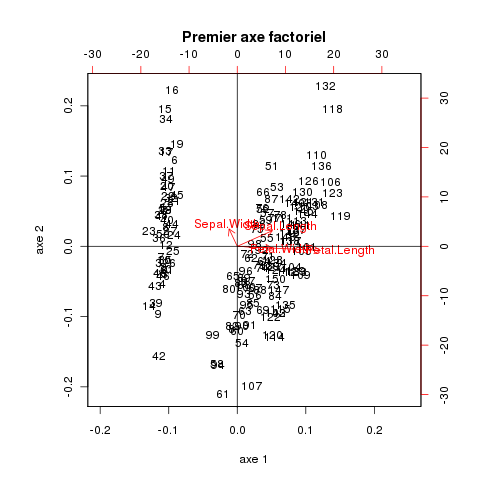
\includegraphics[height = 8cm, width = 8cm]{plots/biplot_axe_factoriel_1.png}\\
On constate que les variables \textit{petal.width} et \textit{petal.length} sont fortement corr\'el\'ees
(ce qui semble logique car ces deux variables sont bas\'ees sur la taille des p\'etales).\\
En revanche, les variables \textit{sepal.width} et \textit{sepal.length} ne sont pas du tout corr\'el\'ees car
nous pouvons observer un angle approchant les 90° entre ces deux variables.
\newpage
\noindent
% QUESTION 1.2
\textbf{Effectuer l'ACP des donn\'ees \textit{Crabs}, pr\'ealablement trait\'ees de mani\`ere \`a supprimer l'effet taille et
comparer \`a la repr\'esentation des Crabes suivant les variables \textit{RW} et \textit{BD}.}\\
% SOLUTION 1.2
Apr\`es traitement des donn\'ees pour supprimer l'effet taille, nous obtenons la repr\'esentation suivantes des donn\'ees :\\
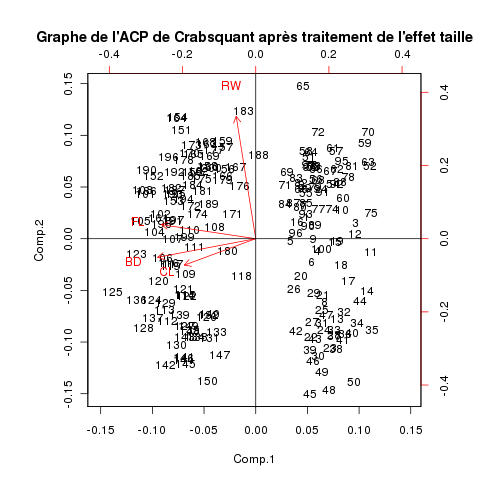
\includegraphics[height = 8cm, width = 8cm]{plots/biplot_axe_factoriel_3.png}
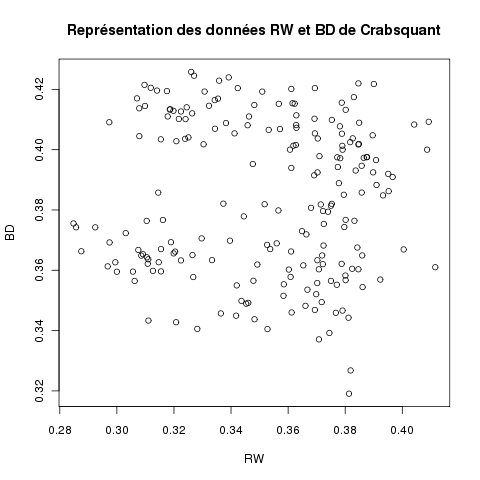
\includegraphics[height = 8cm, width = 8cm]{plots/plot_crabsquant_bd_rw.png}\\
Gr\^ace \`a ces deux graphiques, nous pouvons dire que les variables RW et BD ne sont pas du tout corr\'el\'ees
car elles forment un angle droit sur la repr\'esentation de l'ACP de Crabsquant apr\`es traitement de l'effet taille.\\
De plus, nous pouvons remarquer sur le deuxi\`eme graphique que les points sont tr\`es \'eparpill\'es et
donc appuient cette non-corr\'elation entre les variables RW et BD.\\ \\ \\
% QUESTION 1.3
\textbf{Effectuer l'AFTD des donn\'ees \textit{Mutations}, puis afficher et analyser la repr\'esentation obtenue.}\\
% SOLUTION 1.3
Le traitement de l'AFTD des donn\'ees Mutations au moyen de diagrammes de Shepard nous donne les repr\'esentations suivantes :\\
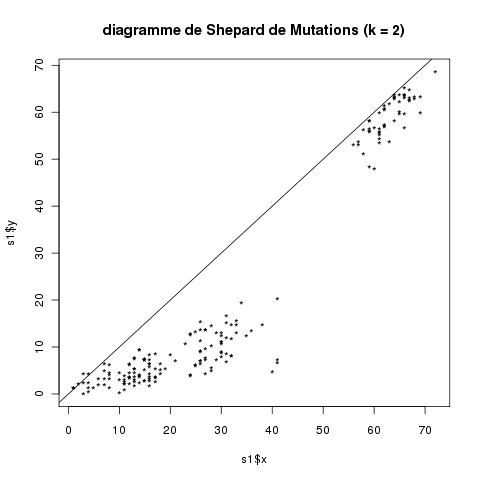
\includegraphics[height = 8cm, width = 8cm]{plots/plot_shepard_1.png}
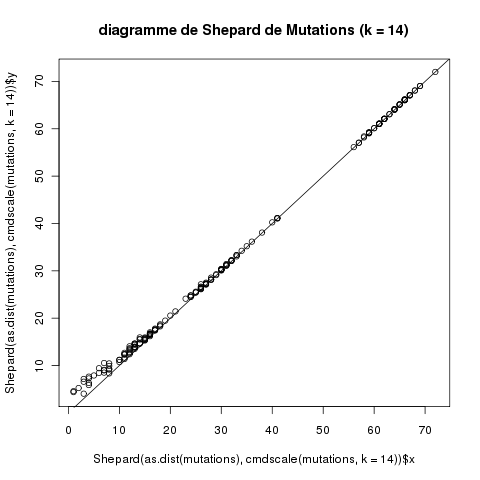
\includegraphics[height = 8cm, width = 8cm]{plots/plot_shepard_2.png}\\
Dans le cas des donn\'ees Mutations, nous utilisons plut\^ot une AFTD au lieu d'une ACP puisque
les donn\'ees sont donn\'ees sour la forme d'une matrice de distances entre esp\`eces.\\
Le diagramme de Shepard sert principalement \`a mesurer l'exactitude entre les distances originales et les distances retrouv\'ees par l'AFTD.\\
Ce diagramme nous permet d'appr\'ecier simplement la qualit\'e des repr\'esentations.
En effet, plus le nuage de points du diagramme est proche de la droite d'\'equation y = x, plus la repr\'esentation est fid\`ele.\\ \\
Nous pouvons donc observer que pour la dimension 2, la repr\'esentation est moins fid\`ele que dans le cas de la dimension 14.\\ \\

\section{Classification hi\'erarchique}
% QUESTION 2.1
\textbf{En utilisant la fonction \textit{hclust}, effectuer la classification hi\'erarchique ascendante
(avec les diff\'erents crit\`eres d'agr\'egation disponibles) des donn\'ees de mutations.
Commenter et\\comparer les r\'esultats obtenus.}\\
% SOLUTION 2.1
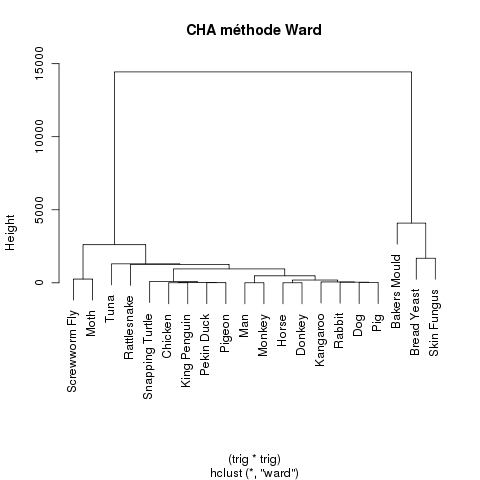
\includegraphics[height = 8cm, width = 8cm]{plots/plot_ward_1.png}
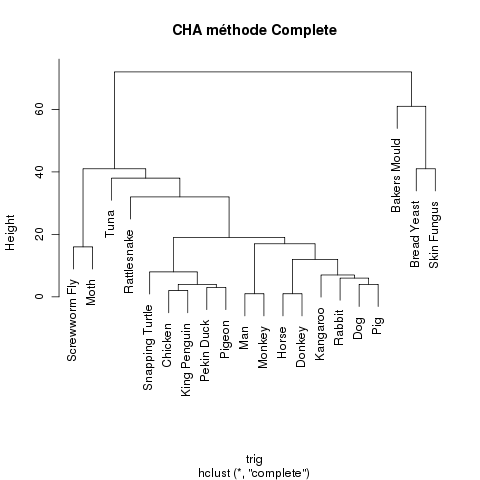
\includegraphics[height = 8cm, width = 8cm]{plots/plot_complete_1.png}\\
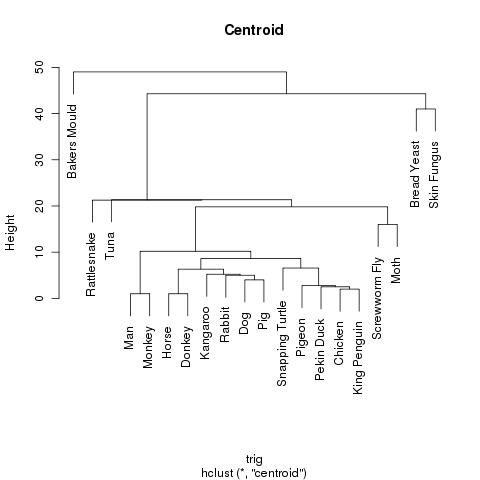
\includegraphics[height = 8cm, width = 8cm]{plots/plot_centroid_1.png}
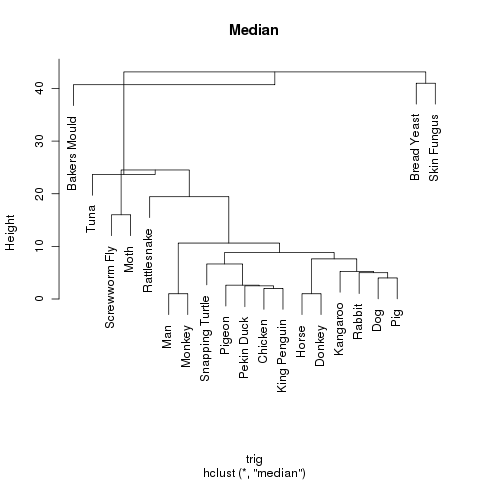
\includegraphics[height = 8cm, width = 8cm]{plots/plot_median_1.png}\\
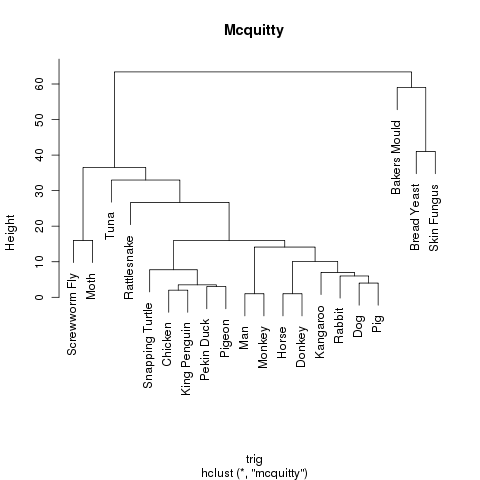
\includegraphics[height = 8cm, width = 8cm]{plots/plot_mcquitty_1.png}
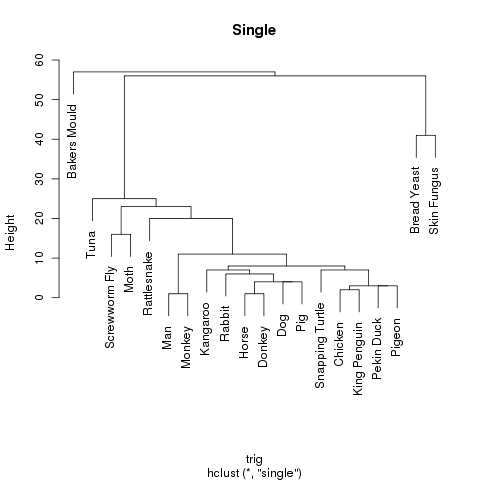
\includegraphics[height = 8cm, width = 8cm]{plots/plot_single_1.png}
\newpage
\noindent
Nous pouvons remarquer que les CAH avec les crit\`eres d'aggr\'egation WARD, Complete, Mcquitty sont similaires.\\
Les CAH avec les crit\`eres d'aggr\'egation Single, Median diff\`erent un peu des 3 premi\`eres.\\
Quant \`a la CAH avec le crit\`ere d'aggr\'egation Centroid, on peut observer une plus nette diff\'erence compar\'e aux 5 autres graphiques.
S'il y en a une à utiliser, il s'agit de la méthode WARD car pour les variables quantitatives,
le crit\`ere de WARD minimise l'inertie intra-classe, ce qui en fait le plus fiable pour notre cas de figure.\\ \\ \\
% QUESTION 2.2
\textbf{Effectuer la classification hi\'erarchique ascendante des donn\'ees \textit{Iris}.
Commenter les r\'esultats obtenus.}\\
% SOLUTION 2.2
Pour effectuer cette CAH, nous utilisons le crit\`ere d'aggr\'egation WARD, ce qui nous donne le\\Dendogramme suivant :\\
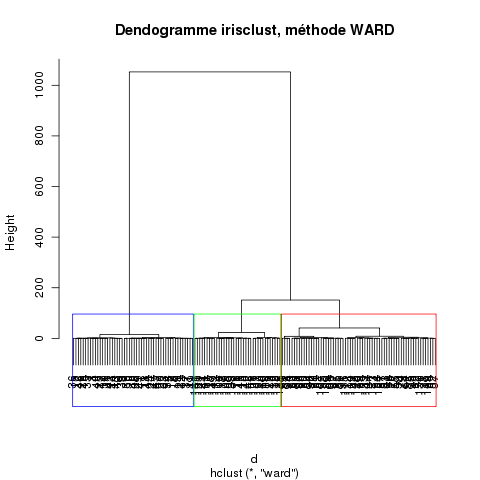
\includegraphics[height = 8cm, width = 8cm]{plots/plot_ward_2.png}\\
Nous avons mis en \'evidence les 3 principaux groupes qui ressortent de ce graphique, qui sont les esp\`eces Setosa, Versicolor et Virginica.\\ \\
Au moyen d'un Clusplot avec le crit\`ere de WARD, nous obtenons la repr\'esentation suivante :\\
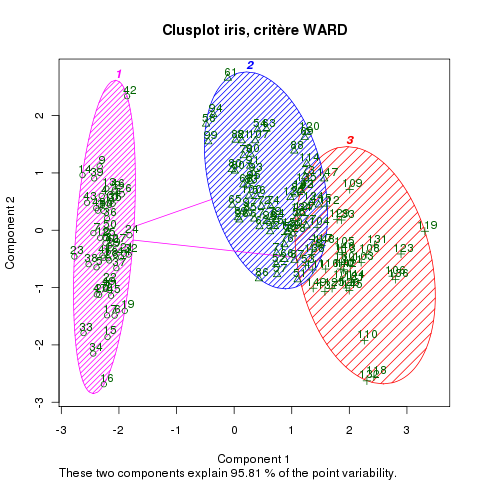
\includegraphics[height = 8cm, width = 8cm]{plots/clusplot_ward_1.png}\\ \\
Cette repr\'esentation nous donne une meilleure vision de la r\'epartition des esp\`eces par rapport au\\Dendogramme.
Nous pouvons observer sur le dernier graphique que les esp\`eces Versicolor et Virginica se chevauchent et donc
peuvent \^etre difficiles \`a diff\'erencier alors que pour reconna\^itre l'esp\`ece Setosa, ce souci ne se pose pas.
\newpage
\noindent 
% QUESTION 2.3
\textbf{Effectuer la classification hi\'erarchique descendante des donn\'ees \textit{Iris}, au moyen de la de la fonction \textit{diana}.
Comparer aux r\'esultats obtenus au moyen de la CAH.}\\
% SOLUTION 2.3
La repr\'esentation de la classification hi\'erarchique descendante des donn\'ees iris nous donne les graphiques suivants :\\
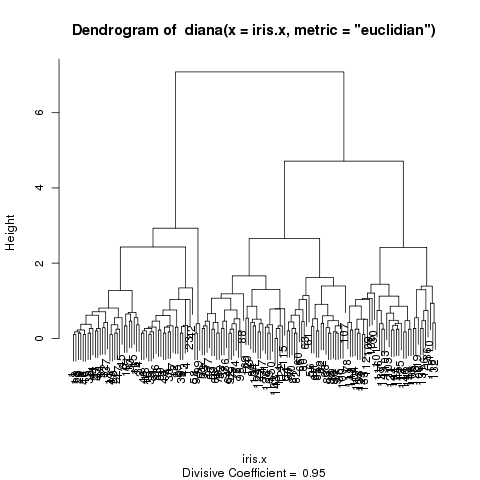
\includegraphics[height = 8cm, width = 8cm]{plots/plot_euclidian_1.png}
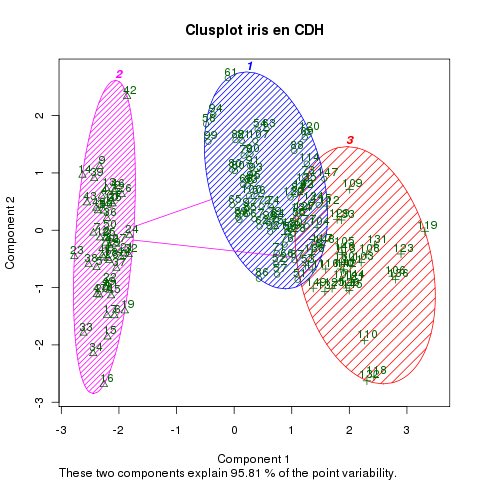
\includegraphics[height = 8cm, width = 8cm]{plots/clusplot_kmeans_10.png}\\ \\
Dans notre cas, nous n'avons pas observ\'e de diff\'erences flagrantes entre les classifications hi\'erarchiques ascendante et descendante.\\ \\ \\

\section{Centres mobiles}
Le but de cet exercice est de tester les performances de l'algorithme des centres mobiles sur deux jeux de donn\'ees r\'eelles :
\textbf{Iris} et \textbf{Crabs}.

\subsection{Donn\'ees Iris}
% QUESTION 3.1
\textbf{Tenter une partition en \textit{K} in \{2,3,4\} classes avec la fonction \textit{kmeans}.
Visualiser et commenter.}\\
% SOLUTION 3.1
En application la fonction \textit{kmeans} sur le jeu de donn\'ees \textbf{iris}, nous obtenons les repr\'esentations suivantes des partitions
demand\'ees :\\
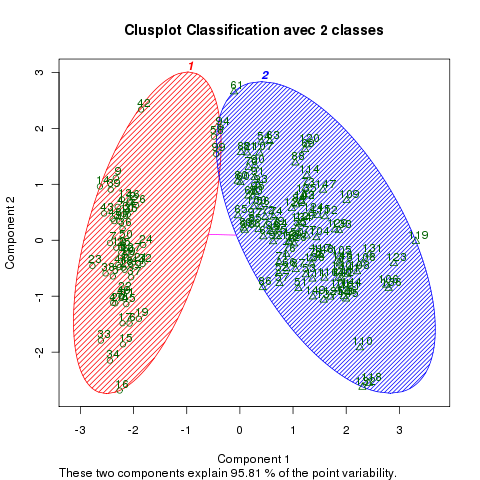
\includegraphics[height = 8cm, width = 8cm]{plots/clusplot_kmeans_1.png}
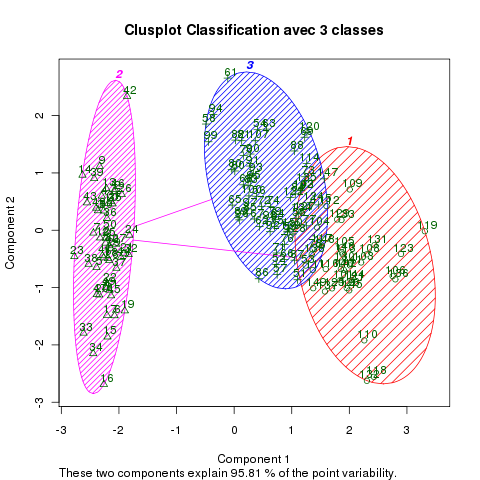
\includegraphics[height = 8cm, width = 8cm]{plots/clusplot_kmeans_4.png}\\
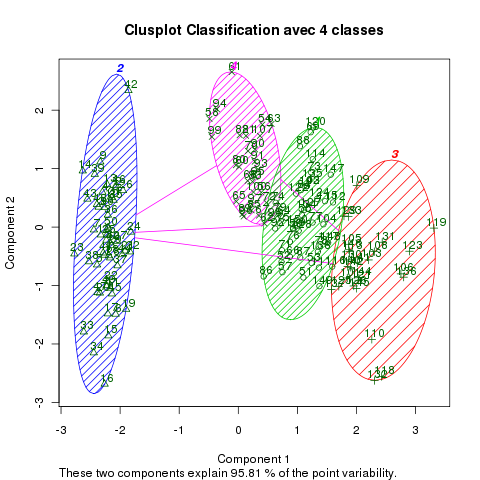
\includegraphics[height = 8cm, width = 8cm]{plots/clusplot_kmeans_3.png}\\ \\
Du fait que le jeu de donn\'ees \textit{iris} regroupe 3 esp\`eces, nous remarquons que la fonction \textit{kmeans} regroupe les esp\`eces Versicolor et Virginica
pour un nombre de classes \'egal \`a 2.\\
Pour un nombre de classes \'egal \`a 4, la fonction \textit{kmeans} se voit contrainte d'inventer un nouveau groupe ne correspondant \`a aucune esp\`ece.\\
Et dans le cas o\`u nous avons 3 classes, nous retrouvons la m\^eme forme de repr\'esentation que
celle \'etudi\'ee pr\'ec\'edemment dans le tp.\\ \\ \\
% QUESTION 3.2
\textbf{\'Etude de la stabilit\'e du r\'esultat de la partition.
Effectuer plusieurs classifications en\\\textit{K} = 3 classes du jeu de donn\'ees.
Observer ces r\'esultats, en termes de classification et d'inertie intra-classes. Les r\'esultats ont-ils chang\'e ? }\\
% SOLUTION 3.2
Nous avons pu remarquer que les r\'esultats diff\'eraient parfois en terme de classification et d'inertie intra-classes comme nous pouvons le voir
sur les repr\'esentations suivantes :\\
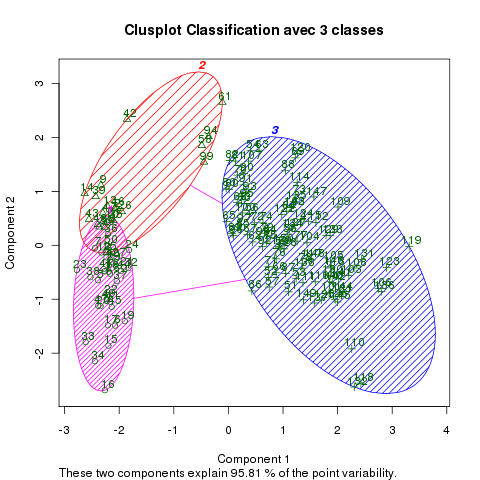
\includegraphics[height = 8cm, width = 8cm]{plots/clusplot_kmeans_2.png}
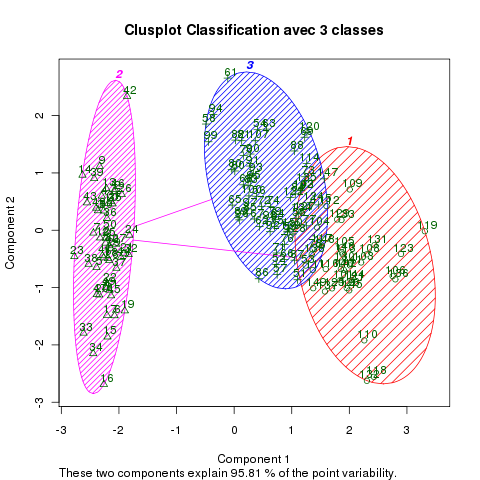
\includegraphics[height = 8cm, width = 8cm]{plots/clusplot_kmeans_4.png}\\ \\
Cette diff\'erence de r\'esultats pour l'ex\'ecution d'une m\^eme instruction provient de l'algorithme de \textit{kmeans} en lui-m\^eme.\\
Cette variation dans les r\'esultats est d\^ue \`a la s\'election al\'eatoire des centres au d\'ebut de l'ex\'ecution du kmeans.
Pour palier \`a ce souci al\'eatoire, nous pouvons indiquer la valeur de d\'epart \`a la fonction \textit{kmeans} avec l'option \textit{nstart = 20}
qui indique \`a la fonction le nombre de points \`a choisir pour avoir le premier centre en d\'ebut d'ex\'ecution de la fonction.
\newpage
\noindent
% QUESTION 3.3
\textbf{On cherche \`a d\'eterminer le nombre de classes optimal.}\\
% SOLUTION 3.3
Afin de rechercher le nombre de classes optimal pour le jeu de donn\'ees iris, nous effectuons\\100 classifications avec un nombre de classes
compris entre 2 et 10, ce qui nous donne 9 \'echantillons contenant chacun 100 valeurs d'inertie intra-classe.\\
Ensuite pour chaque valeur de classe, nous calculons l'inertie intra-classe minimale et nous repr\'esentons sa variation
en fonction du nombre de classes :\\
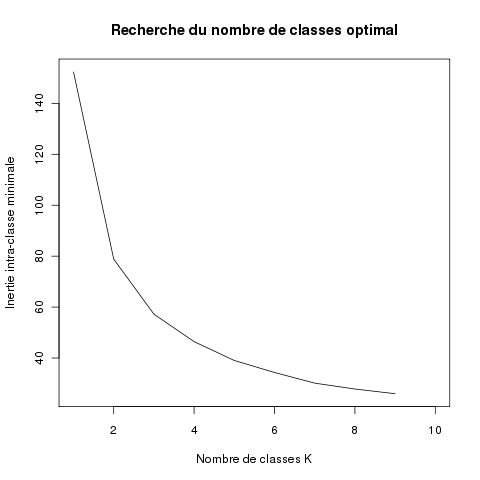
\includegraphics[height = 6cm, width = 8cm]{plots/plot_inertie_intra_1.png}\\ \\
Pour d\'eterminer le nombre de classe optimal \`a partir de cet repr\'esentation des variations de l'inertie intra-classe minimale,
nous utilisons la m\'ethode du coude qui nous indique que le nombre de classes\\optimal est \'egal \`a soit 2, soit 3,
mais nous avons pr\'ef\'erez prendre la valeur 3 qui est plus coh\'erente vis-\`a-vis du nombre d'esp\`eces disponibles dans
le jeu de donn\'ees \textit{iris}.\\ \\ \\
% QUESTION 3.4
\textbf{Comparer les r\'esultats de la partition obtenue par les centres mobiles avec la partition r\'eelle des iris en trois groupes.}\\
% SOLUTION 3.4
Nous avons compar\'e les partitions obtenues par les centres mobiles et r\'eelles des iris :\\
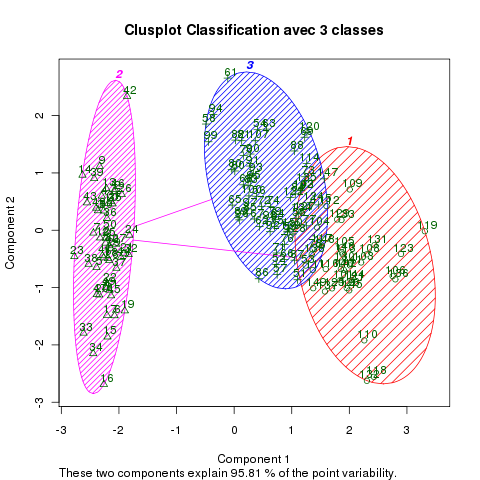
\includegraphics[height = 8cm, width = 8cm]{plots/clusplot_kmeans_4.png}
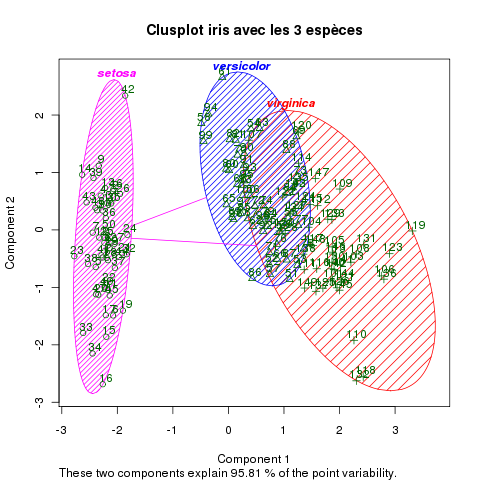
\includegraphics[height = 8cm, width = 8cm]{plots/clusplot_iris_10.png}\\ \\
Nous avons pu observer que les 2 repr\'esentations sont similaires, l'esp\`ece Setosa est bien identifi\'ee dans les 2 cas tandis que
des valeurs des esp\`eces Versicolor et Virginica se recoupent.\\ \\ \\

\newpage
\subsection{Donn\'ees Crabs}
% QUESTION 3.5
\textbf{Effectuer la classification des donn\'ees \textit{Crabs} au moyen de l'algorithme des centres mobiles.
Comparer \`a la partition r\'eelle des crabes suivant l'esp\`ece et le sexe.}\\
% SOLUTION 3.5
Dans un premier temps, nous r\'ecup\'erons puis traitons les donn\'ees pour supprimer la forte corr\'elation pr\'esente dans le jeu de donn\'ees
crabs entre les variables.\\
Ensuite nous nous resservons du travail effectu\'e en amont pour d\'eterminer le nombre de classes optimal pour ce jeu de donn\'ees :\\
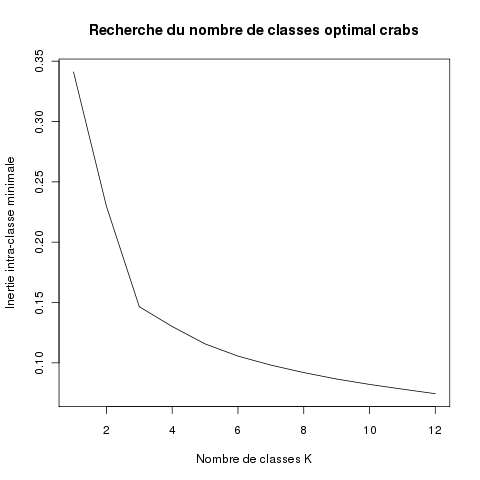
\includegraphics[height = 6cm, width = 8cm]{plots/plot_inertie_intra_2.png}\\ \\
Nous remarquons sur ce graphique que la m\'ethode du coude rel\`eve que le nombre de classes optimal est \'egal \`a 3 et
la pr\'esence de coudes pour les valeurs 2 et 4 n'est pas assez prononc\'ee.\\
Cela signifie peut \^etre qu'une erreur de manipulation sur les donn\'ees a \'et\'e effectu\'ee mais
nous avons remarqu\'e que sur les repr\'esentations des sexes et des esp\`eces, les valeurs, pour les esp\`eces, \'etaient bien s\'epar\'ees
mais que dans certains cas pour les sexes, les valeurs \'etaient m\'elang\'ees :\\
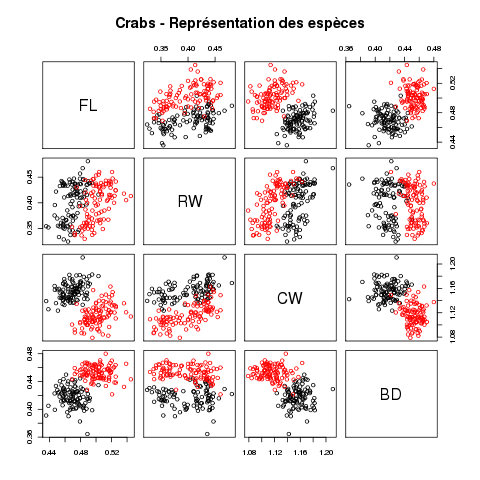
\includegraphics[height = 6cm, width = 6cm]{plots/plot_crabs_sp_2.png}
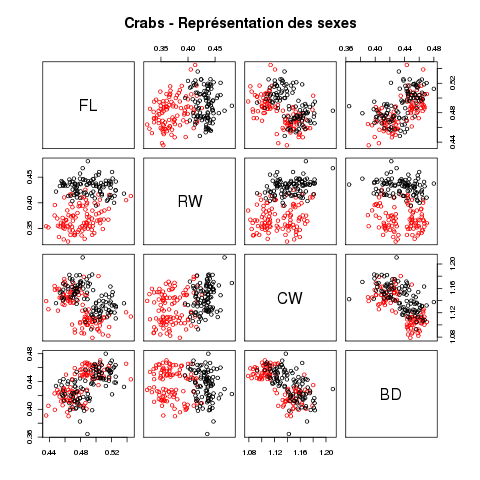
\includegraphics[height = 6cm, width = 6cm]{plots/plot_crabs_sex_2.png}\\ \\
Cela pourrait expliquer le fait que le nombre de classes optimal soit \'egal \`a 3 au lieu de 4.\\
Les repr\'esentations de la classification du donn\'ees de jeu Crabs pour K = 2 et K = 3 sont les suivantes :\\
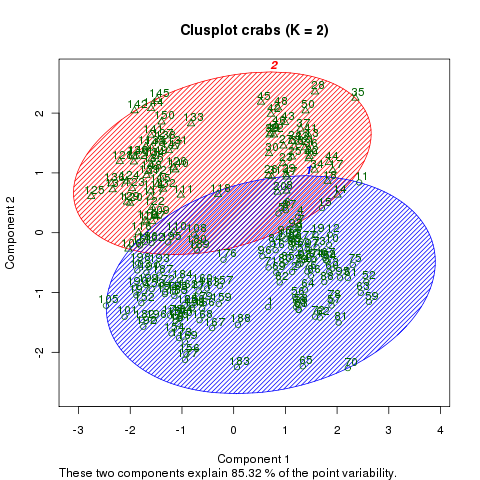
\includegraphics[height = 7cm, width = 7cm]{plots/clusplot_crabs_10.png}
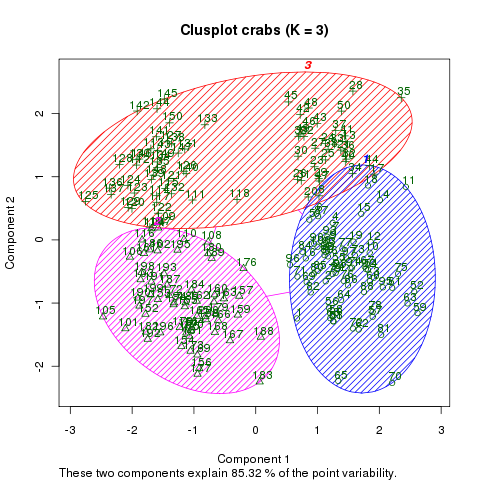
\includegraphics[height = 7cm, width = 7cm]{plots/clusplot_crabs_11.png}\\ \\
Mais pour comparer la classification du donn\'ees de jeu Crabs \`a la partition r\'eelle, nous avons tout de m\^eme pr\'ef\'er\'e nous baser
sur un nombre de classes optimal \'egal \`a 4 :\\
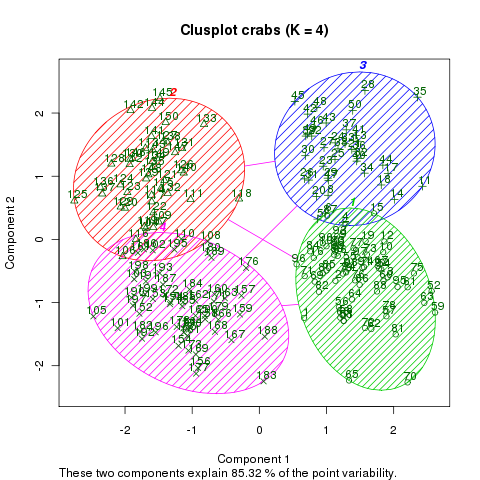
\includegraphics[height = 8cm, width = 8cm]{plots/clusplot_crabs_12.png}
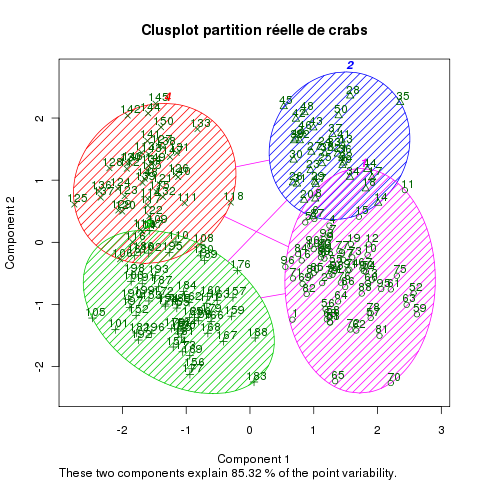
\includegraphics[height = 8cm, width = 8cm]{plots/clusplot_crabs_13.png}\\ \\
L'\'etude de ces 2 graphiques nous montre que la classification du jeu de donn\'ees crabs semble juste m\^eme si nous pouvons remarquer
que les cercles ont tendance \`a se chevaucher 2 \`a 2 dans les deux\\partitions.\\ \\ \\

\section*{Conclusion}
Les exercices de ce TP nous ont donc permis de d\'ecouvrir plusieurs techniques de classification\\automatique telles que
les classifications hi\'erarchiques ascendante et descendante et ainsi que la m\'ethode des centres mobiles.\\
Ce TP nous a surtout permis de conna\^itre les \'el\'ements importants pour l'utilisation de ces outils de classification automatique.

\end{document}
